\large \bf{\textsc{\section{Lab 4}}
	\begin{problem}
		Using an OpAmp TL082, construct an amplifier that can deliver the following functions. Evaluate your circuit practically and theoretically.
		\newline
		1. z = 0.2x + y\\
		2. z = 3(x-y)\\
	\end{problem}
	
	\begin{solution}
		1. R$_{1}$= 1.8k\(\Omega\), R$_{2}$= 8.2k\(\Omega\), R$_{3}$= 1.8k\(\Omega\), Gain = 0.2, v$_{1}$= 5V, v$_{2}$= 5V
		
		\begin{figure}[h!]
			\centering
			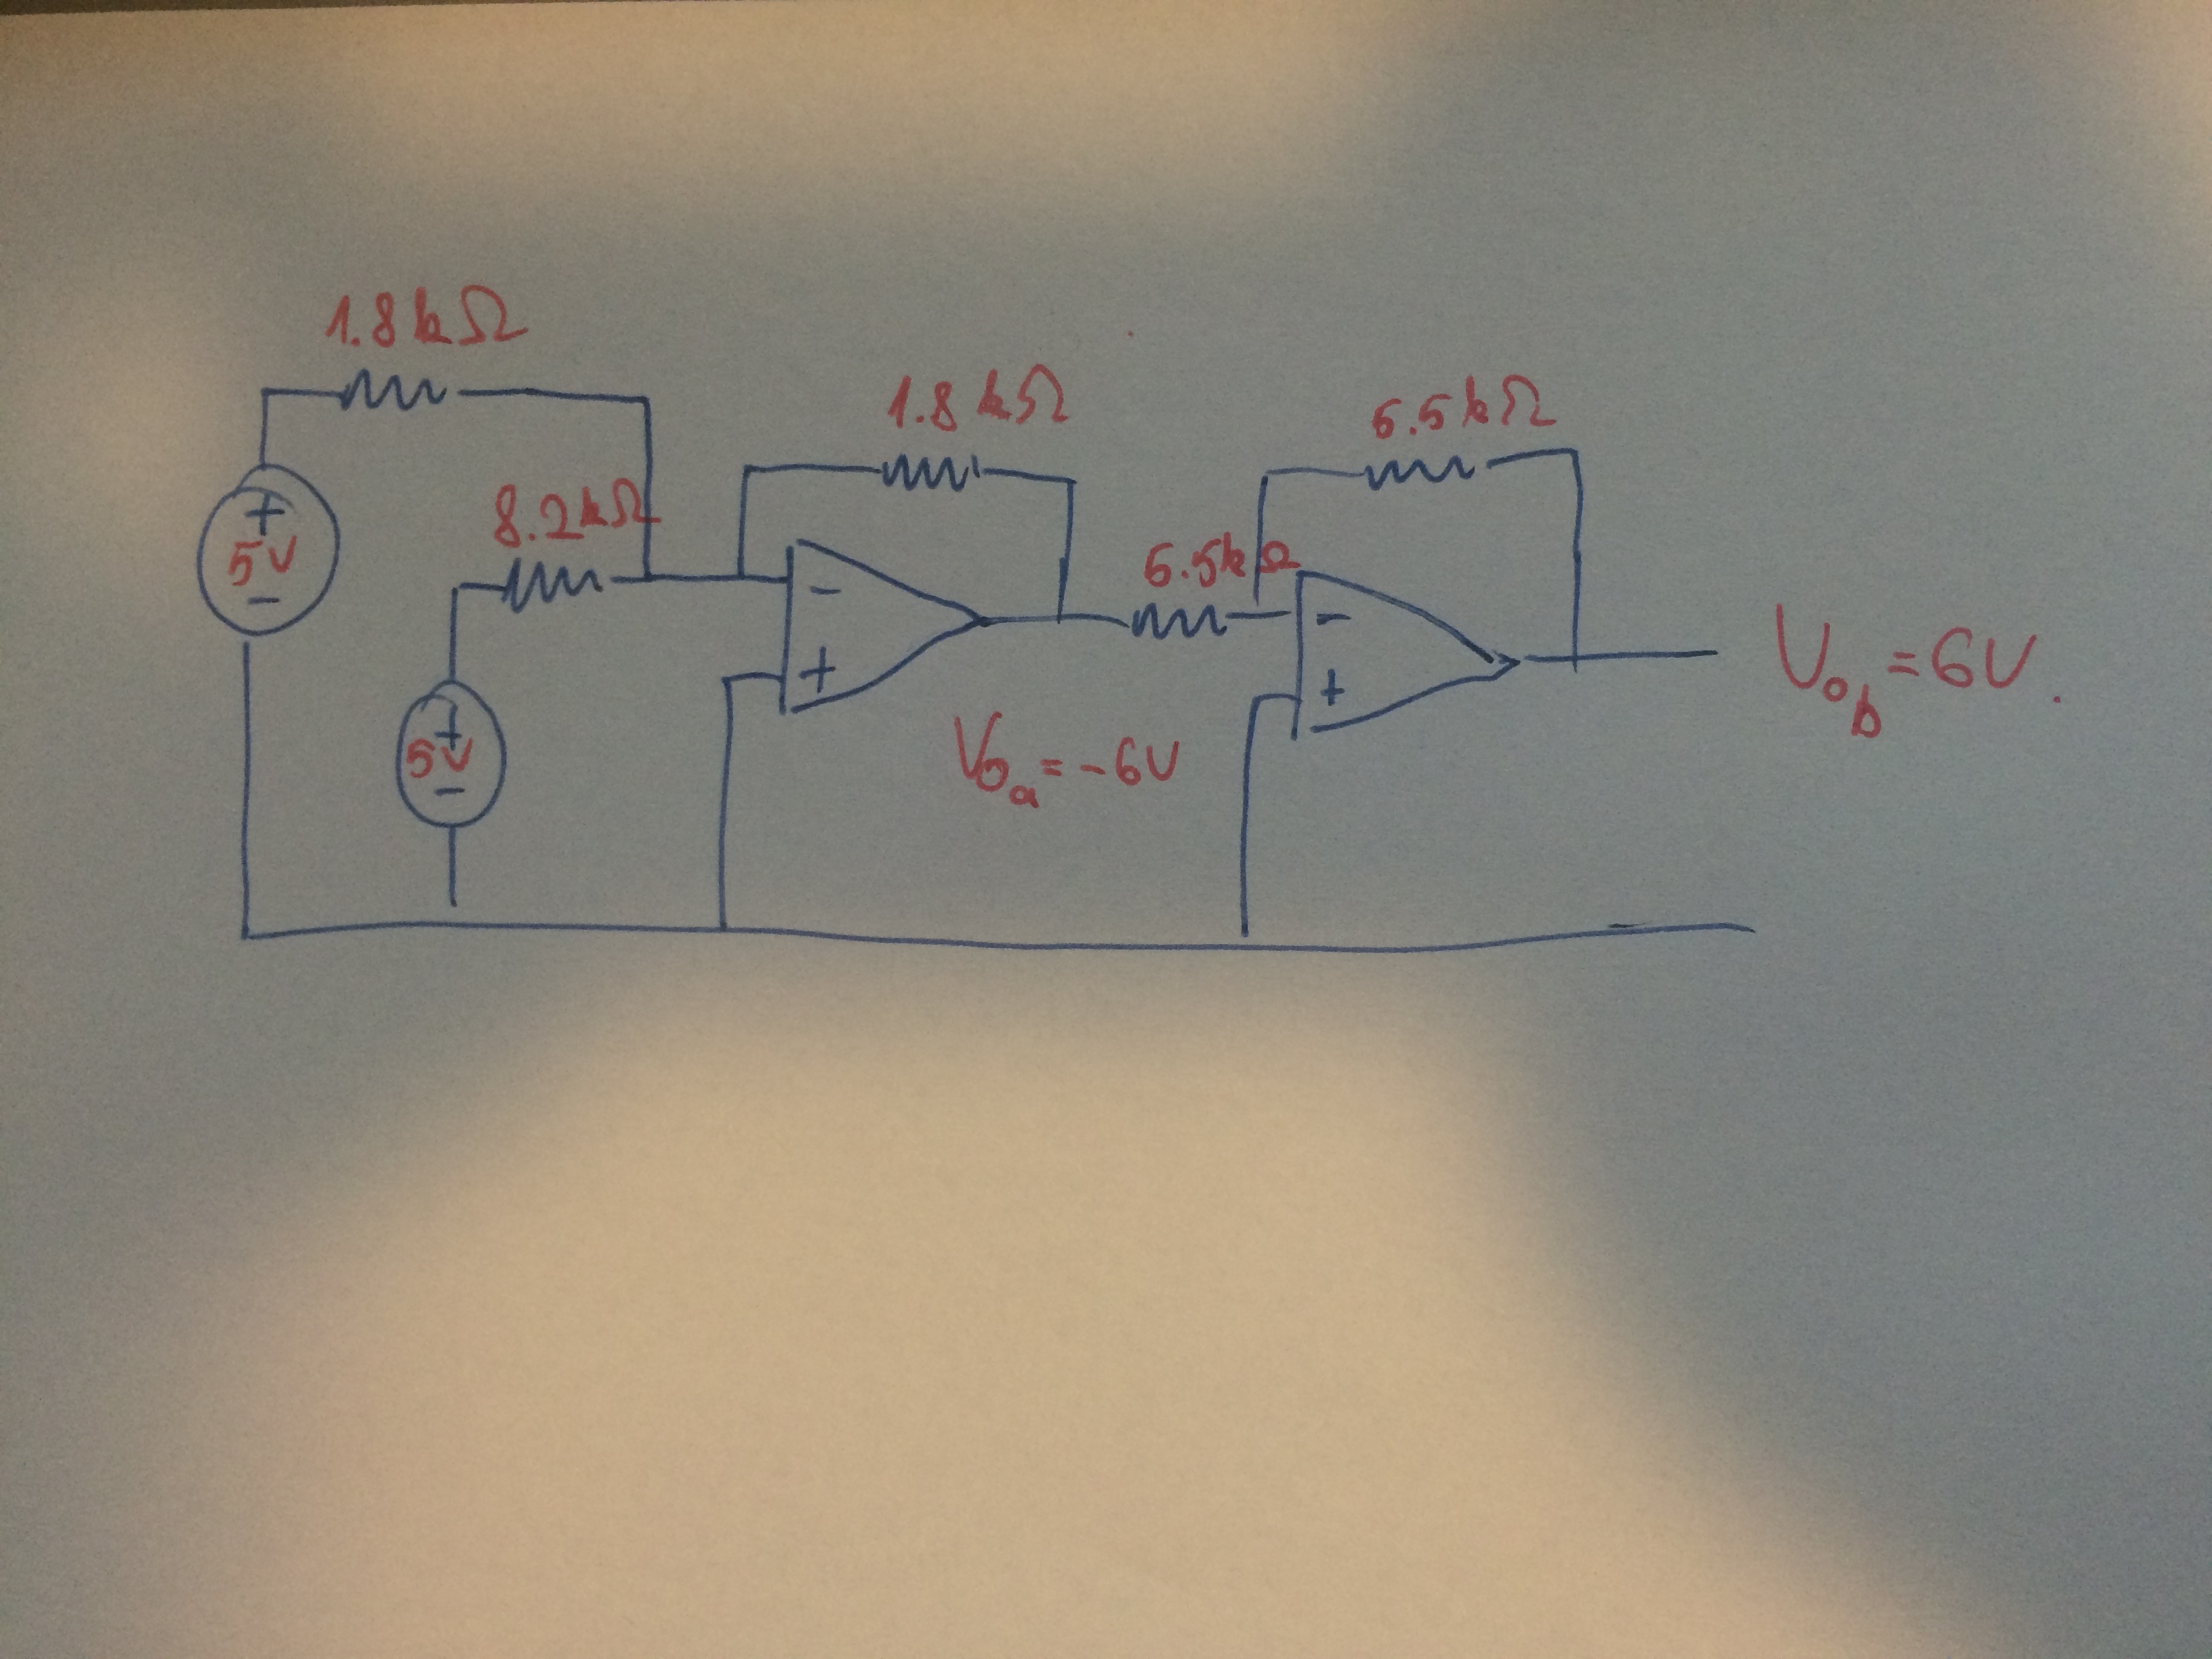
\includegraphics[width=0.4\textwidth]{images/circuit411.jpg}
		\end{figure}
		
		This is an adder, therefore we used the following formula:
		\newline
		v$_{o}$\(\approx\)$-(R_{3}/R_{1}*v_{1} + R_{3}/R_{2}*v_{2})$
		
		
		$-((1.8/1.8)*5+(1.8/8.2)*5)=-6$
\\ \\ \\
		2. R$_{1}$=R$_{3}$= 3.3k\(\Omega\), R$_{2}$=R$_{4}$ 10k\(\Omega\), Gain = 3, v$_{1}$= 5V, v$_{2}$= 3V
		
		\begin{figure}[h!]
			\centering
			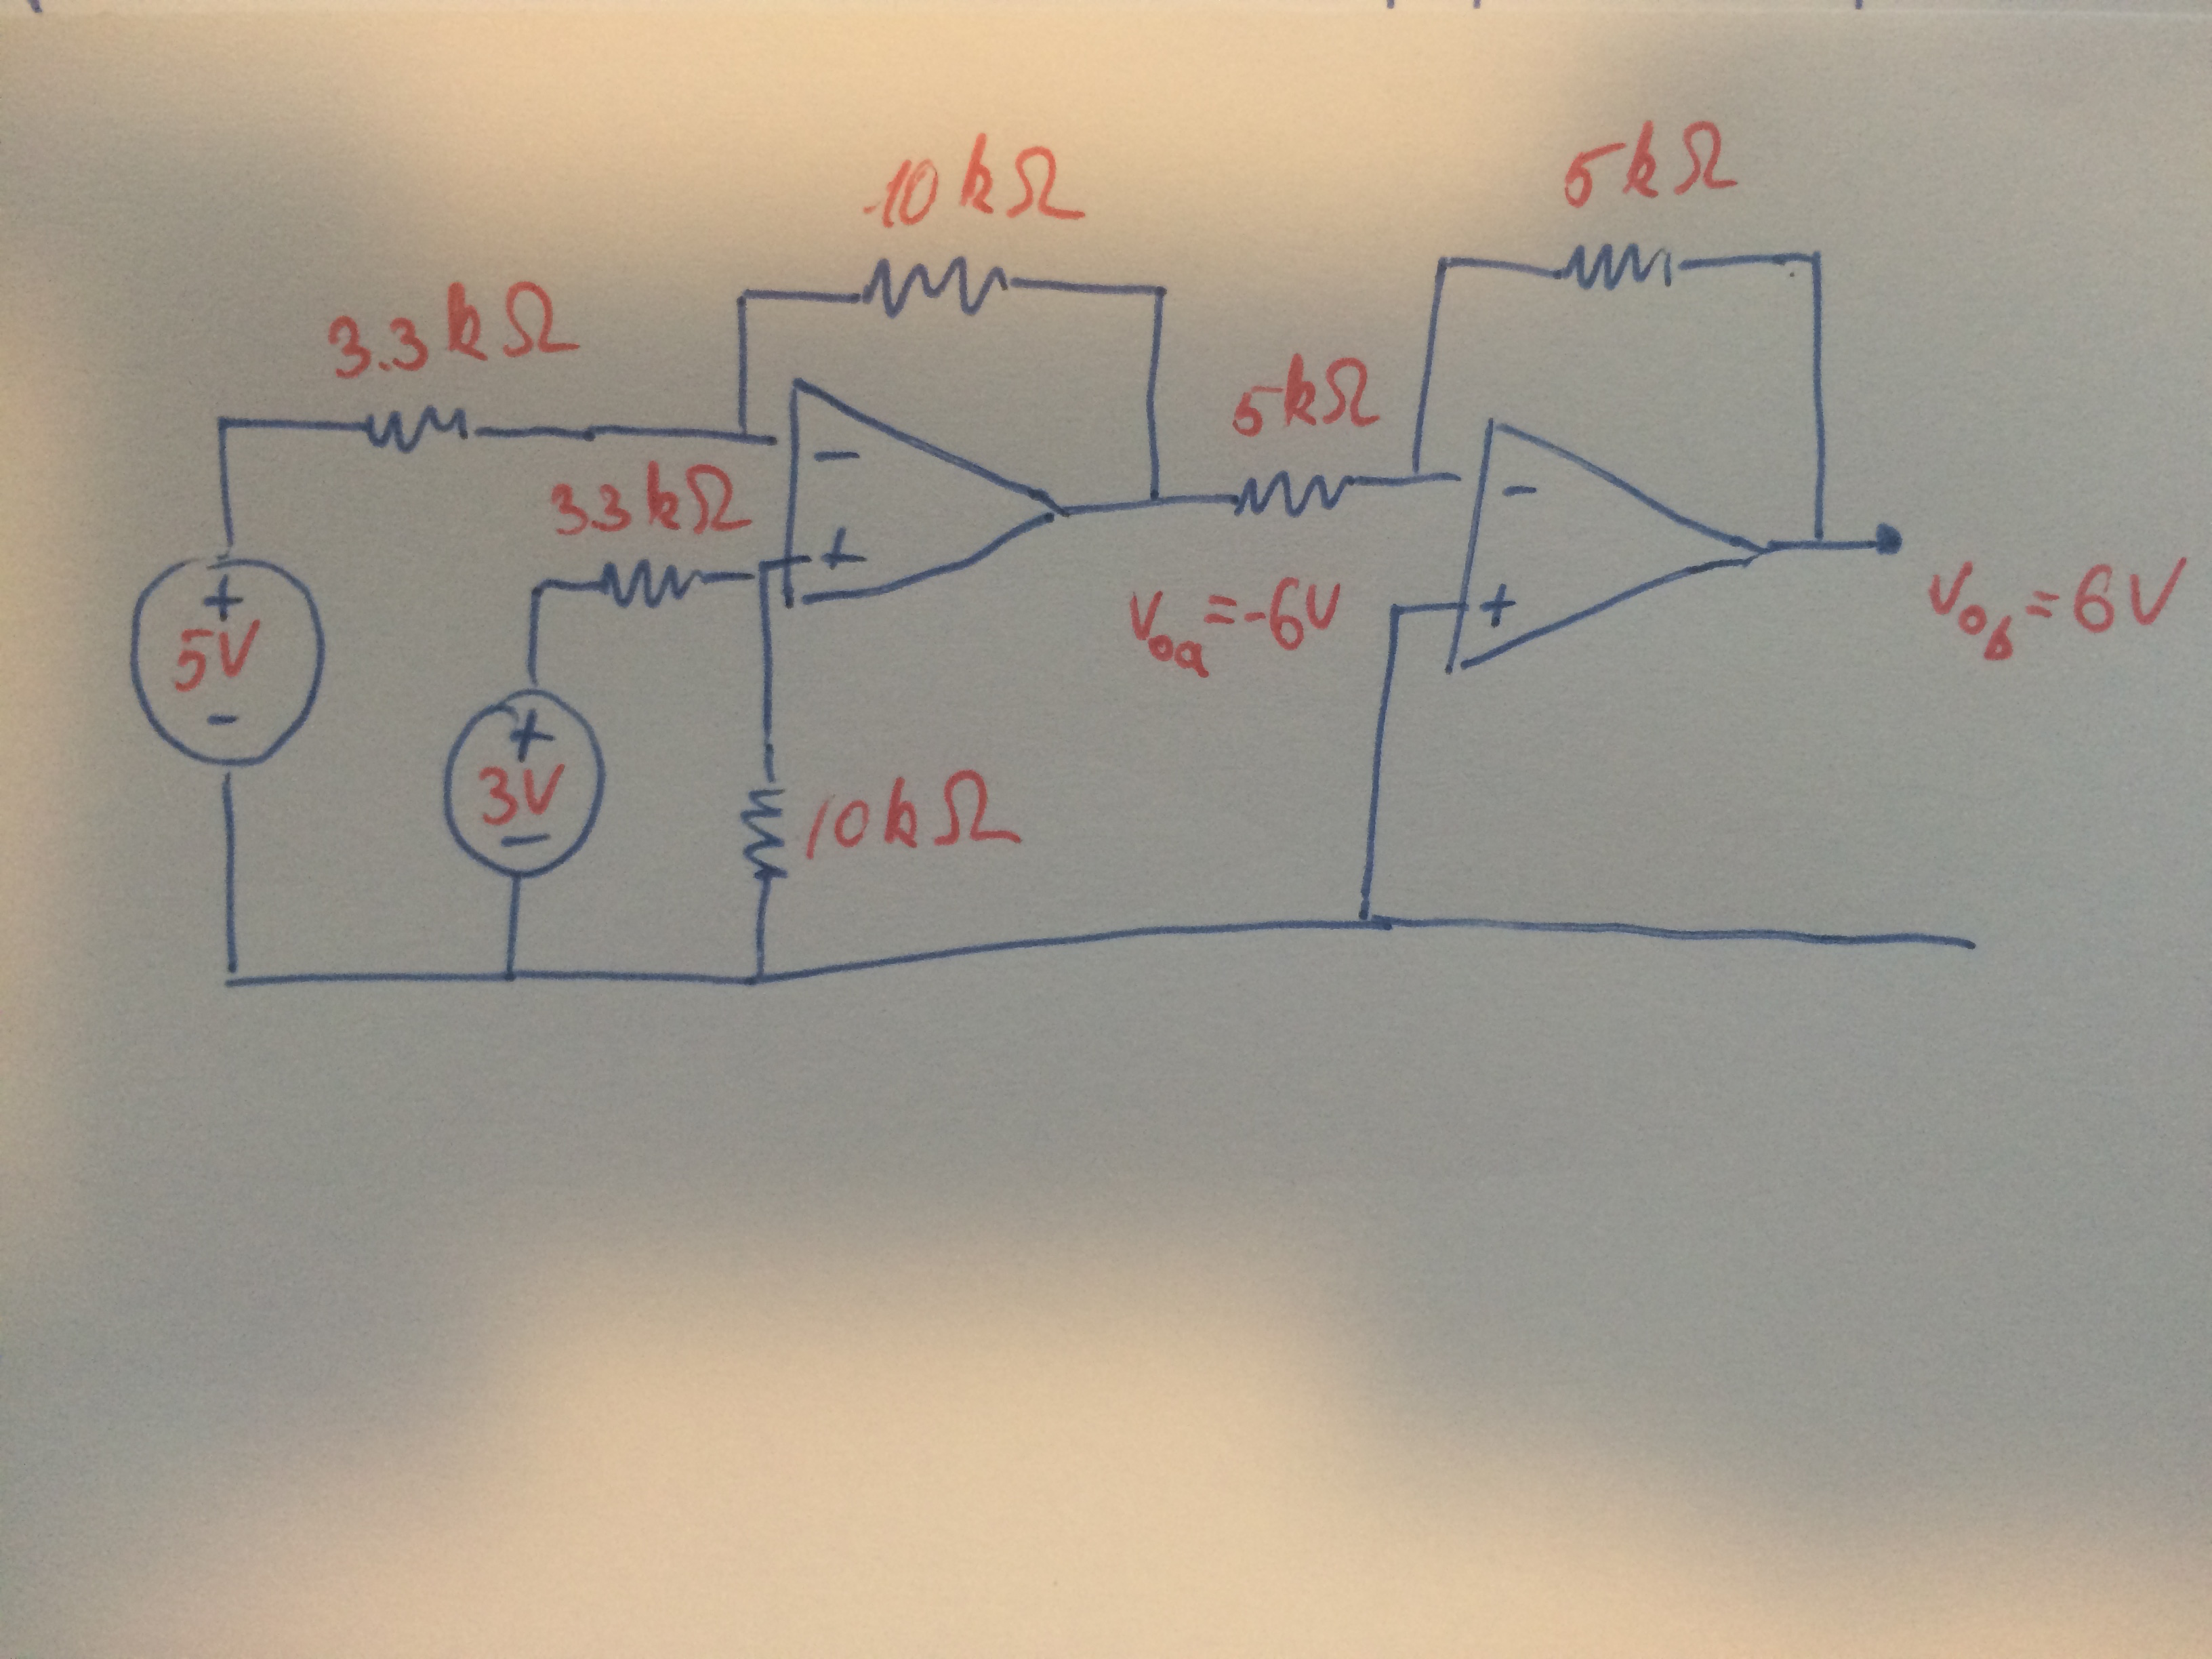
\includegraphics[width=0.4\textwidth]{images/circuit412.jpeg}
		\end{figure}
		
		This was a subtracter, therefore we used the following formula:
		\newline
		$v_{o}=(R_{2}/R_{1})*(v_{2}-v_{1})$
		
		$(10/3.3)*(3-5)=-6$
	\end{solution}
	\clearpage
	\begin{problem}
		We would like to investigate the properties of the MOSFET type BS170. Construct the following circuit with R=1K\(\Omega\). (a and b are equivalent)
\iffalse
		\begin{figure}[h!]
			\centering
			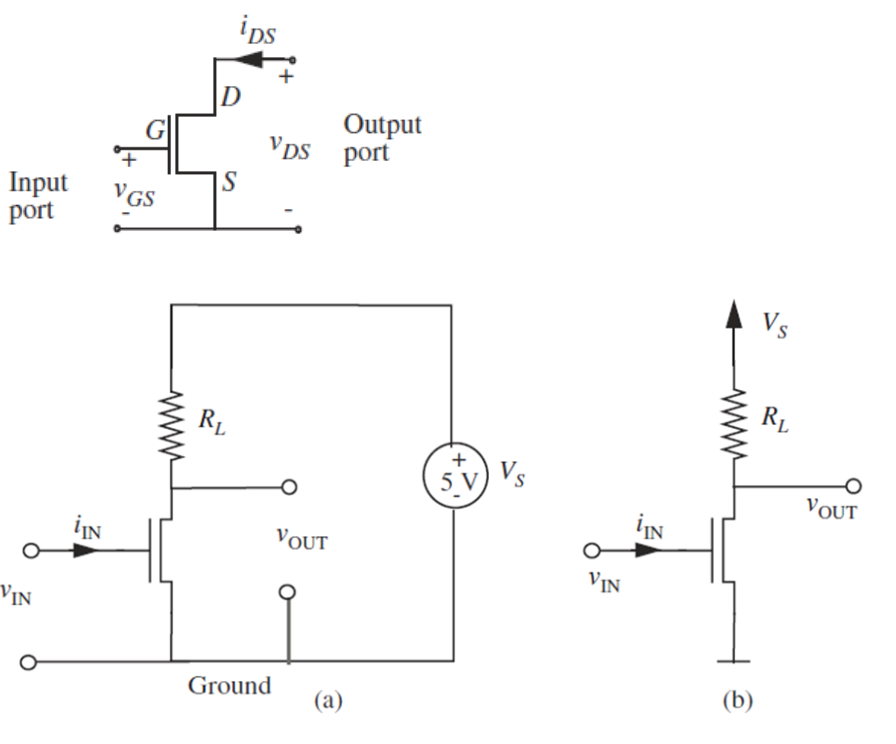
\includegraphics[width=0.4\textwidth]{images/circuit4.png}
		\end{figure}
\fi
		\newline
		1. Measure the V\(_{out}\) and i\(_{DS}\) for the MOSFET for different values of V\(_{IN}\) and fill the table.
		\newline
		2. Plot your input-output characteristics of the MOSFET. What is the treshold voltage V\(_{T}\) for V\(_{GS}\)? Compare your findings with the datasheet.
		\newline
		3. Measure the V\(_{DS}\) and i\(_{DS}\) for the MOSFET for different values of V\(_{S}\) and fill the table once the MOSFET is on.
		\newline
		4. Plot the I-V characteristics of the MOSFET and obtain R\(_{ON}\). Compare your findings with the datasheet.
	\end{problem}
	
	\begin{solution}
		1. 		
		\begin{table}[h!]
			\begin{tabular}{| l | l | l | l | l | l | l | l | l | l | l | l |}
				\hline
				Try & 1 & 2 & 3 & 4 & 5 & 6 & 7 & 8 & 9 & 10 & 11 \\ \hline
				V$_{OUT}$ (V) & 5 & 5 & 4.965 & 4.827 & 3.980 & 1.090 & 0.057 & 0.025 & 0.019 & 0.010 & 0.008 \\ \hline
				V$_{IN}$ (V) & 0 & 1 & 1.9 & 2.1 & 2.3 & 2.5 & 2.7 & 2.9 & 3 & 4 & 5 \\ \hline
			\end{tabular}
		\end{table}
		\newline
		2.
		The gate threshold level is between 2.1 V and 2.7 V. This value fits well into the minimum and maximum voltage values specified on the MOSFET BF170 datasheet, which is 0.8V and 3V.
		\newline
		3.
		\begin{table}[h!]
			\begin{tabular}{| l | l | l | l | l | l | l | l | l | l | l | l |}
				\hline
				Try & 1 & 2 & 3 & 4 & 5 & 6 & 7 & 8 & 9 & 10 & 11 \\ \hline
				V$_{DS}$ (V) & 0.008 & 0.010 & 0.011 & 0.013 & 0.014 & 0.016 & 0.018 & 0.019 & 0.021 & 0.022 & 0.024 \\ \hline
				V$_{S}$ (V) & 5 & 6 & 7 & 8 & 9 & 10 & 11 & 12 & 13 & 14 & 15 \\ \hline
				i$_{DS}$ (mA) & 5 & 6 & 7 & 8 & 9 & 10 & 11 & 12 & 13 & 14 & 15 \\ \hline
			\end{tabular}
		\end{table}
		\newline
		4.The trend function of the chart 4.2.4 is $y = 1.582 * x + 1.818$, therefore we can calculate R$_{ON}$ is 1/1.818\(\approx\)0.6 which is the half of what the datasheet says. The R$_{ON}$, also called R$_{DS}$ on the datasheet, is 1.2 \(\Omega\) with a 10V drain-source and 200mA i$_{DS}$. Because we use 5V, instead of 10V, we find the obtained R$_{ON}$ data acceptable and within limits.
		\newline
		\begin{figure}[h!]
			\begin{subfigure}[H]{0.5\textwidth}
				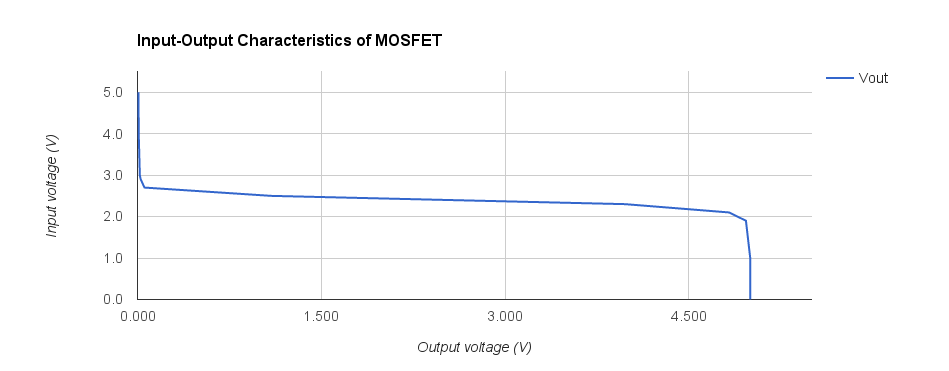
\includegraphics[width=1\textwidth]{images/plot422.png}
				\subcaption{4.2.2}
			\end{subfigure}
			\begin{subfigure}[H]{0.7\textwidth}
				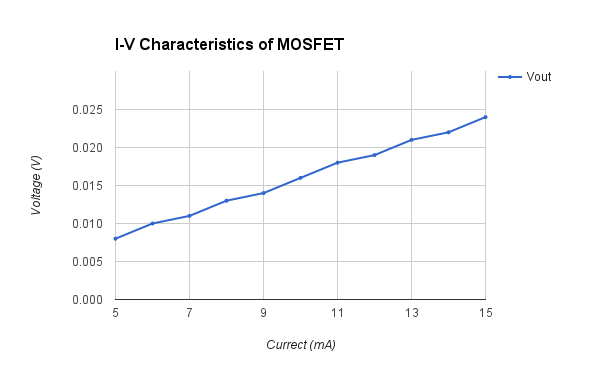
\includegraphics[width=0.8\textwidth]{images/plot424.png}
				\subcaption{4.2.4}
			\end{subfigure}
		\end{figure}
	\end{solution}
	\clearpage
	\begin{problem}
		Using MOSFET type BS170, construct circuits that represent the following logic functions. Evaluate your circuit practically and theoretically.
		\newline
		1. A+B+C \\
		2. A.B+\(\overline{C}\) \\
		3. A.B+C \\
		4. \(\overline{A.\overline{B}+\overline{C}}\)
	\end{problem}
	
	\begin{solution}
		\begin{figure}[h!]
			\centering
			\begin{subfigure}[H]{0.4\textwidth}
				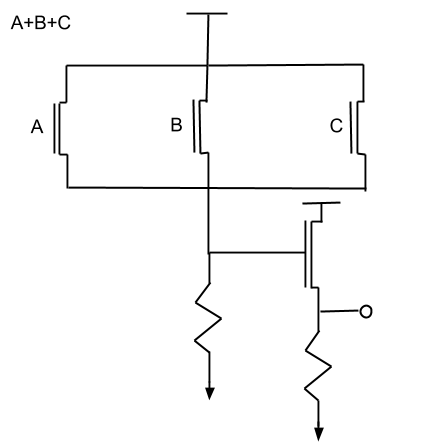
\includegraphics[width=\textwidth]{images/solution431.png}
				\subcaption{4.3.1}
			\end{subfigure}
			\begin{subfigure}[H]{0.4\textwidth}
				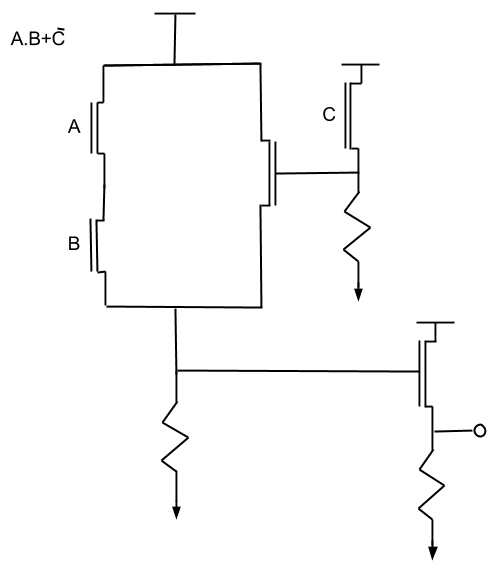
\includegraphics[width=\textwidth]{images/solution432.png}
				\subcaption{4.3.2}
			\end{subfigure}
			\quad
			\begin{subfigure}[H]{0.4\textwidth}
				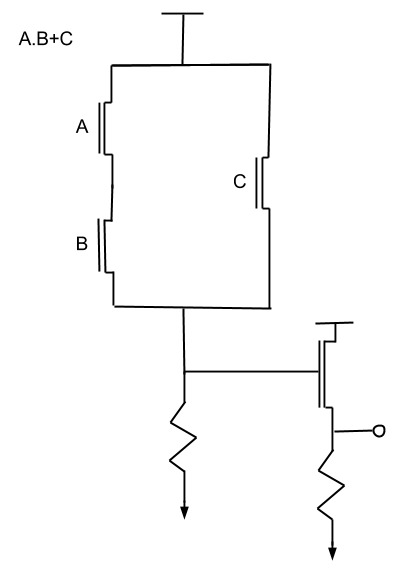
\includegraphics[width=\textwidth]{images/solution433.png}
				\subcaption{4.3.3}
			\end{subfigure}
			\begin{subfigure}[H]{0.4\textwidth}
				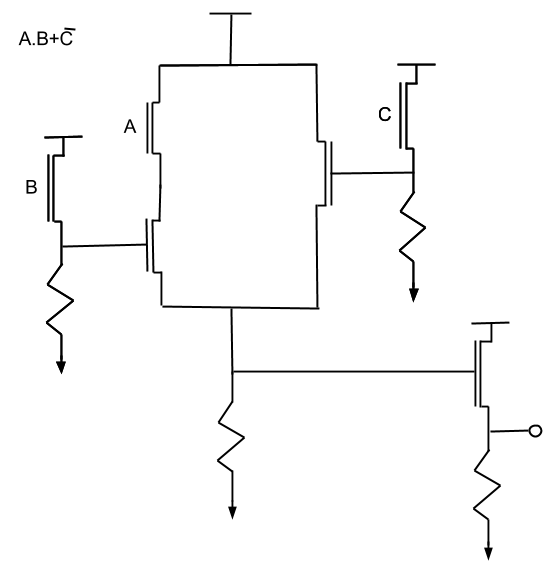
\includegraphics[width=\textwidth]{images/solution434.png}
				\subcaption{4.3.4}
			\end{subfigure}
		\end{figure}
	\end{solution}